\documentclass[12pt]{article}
\usepackage{tikz}
\usepackage{amsmath}
\usepackage{float}
\usepackage{caption}
\usepackage{array}
\usepackage{cancel}

\title{Adding and Subtracting Course\\
\begin{center}

\includegraphics[width=4em]{ApS_logo.png}
\end{center}
\begin{normalsize}Applied Scholastics, Ferndale \end{normalsize}}
\author{}
\date{}

\begin{document}
\maketitle


\section*{Addition}

\paragraph{Addition}
Addition means combining things together into one single amount.\\

The addition of 5 things $\otimes\otimes\otimes\otimes\otimes$ to two things $\otimes\otimes$ gives you 7 things $\otimes\otimes\otimes\otimes\otimes\otimes\otimes$.

\paragraph{Adding}
Adding just means doing addition.\\

If you have 3 of something, $\otimes\otimes\otimes$, adding 2 more of them, $\otimes\otimes$, makes a group of 5 things, $\otimes\otimes\otimes\otimes\otimes$.

\paragraph{Add}
To add also just means doing addition.\\

If you add two $\otimes\otimes$ and six $\otimes\otimes\otimes\otimes\otimes\otimes$ you get eight $\otimes\otimes\otimes\otimes\otimes\otimes\otimes\otimes$.

\begin{enumerate}

\item What is addition, in your own words?
\item What is adding, in your own words?
\item What does add mean, in your own words?
\item Write 3 sentences using the word addition.
\item Write 3 sentences using the word adding.
\item Write 3 sentences using the word add.

\paragraph{Plus}
Plus means "and"  or "more" and in writing addition, the plus sign "+" is used. The "+" sign is from the Latin word "et," which means "and," changed in shape a bit over the years.\\

\item What does plus mean, in your own words?
\item Write 3 sentences using the word plus.

\paragraph{Augend}
The first number is called the augend, from Latin meaning "to increase."

\paragraph{Addend}
The number being added to it is the addend, from Latin meaning "put to."

You wont use these words often, but knowing them can make addition easier to talk about when you need to be specific about which number you mean.\\

\item What is an augend?
\item Write 3 sentences using the word augend.
\item What is an addend?
\item Write 3 sentences using the word addend.
\item Why might you want to know the words augend and addend?

\paragraph{Sum} The amount that you have when you add two things together is called their sum. You would say 'the sum of 32 and 16 is 48.'

Also, the whole thing can be called a sum. Even other arithmetic problems than addition are called sums. That's why arithmetic, and not just adding, is sometimes called 'doing sums.'

\begin{table}[H]
    \centering
    \begin{tabular}{ccccc}
     \   & plus &   \    & equals &  \ \\
     \large{2}   &  \large{+}   &   \large{3}    &   \large{=}    &  \large{5} \\
  augend &  \   & addend &   \    & sum
    \end{tabular}
\end{table}

\item What is a sum?
\item Write 3 sentences using the word sum.

\paragraph{Total} Total also means the amount that you have when you add things together, but total is the word to use for adding lots of things together, not just two things. You might say, 'we collected a total 328 cans this week.'

\begin{table}[H]
    \centering
    \begin{tabular}{ccccccc}
     \   & plus &   \    & plus &   \    & equals & \  \\
     \large{2}   &  \large{+}   &   \large{3}    &   \large{+}  &   \large{4}    &   \large{=}    &  \large{9} \\
  augend &  \   & addend &   \  & addend &   \    & total
    \end{tabular}
\end{table}

\item What is a total?
\item Write 3 sentences using the word total.

\paragraph{Number Lines}
You can think of numbers as being evenly spaced points along a line. A number line is a way of showing what is happening with addition. Moving to the right on the line represents adding.\\

Here is a number line showing $2+3=5$:

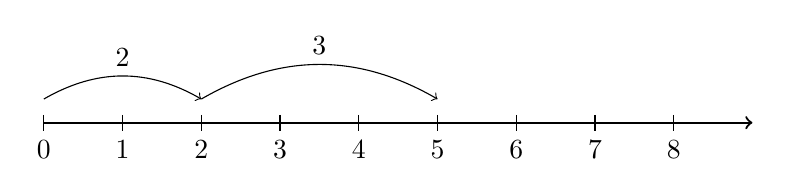
\begin{tikzpicture}
\draw[thick, ->] (0,0) -- (9,0) node[below] {$\ $};
\foreach \n in {0,1,2,3,4,5,6,7,8} {\draw (\n,0.1) -- (\n,-0.1) node[below] {$\n$};}
\draw[->, bend left=30] (0,0.3) to node[above] {$2$} (2,0.3);
\draw[->, bend left=30] (2,0.3) to node[above] {$3$} (5,0.3);
\end{tikzpicture}

\item Draw a number line showing 3 plus 4.
\item From your number line, what is the sum of 3 and 4?

\paragraph{The Addition Table}
Learning to add starts with memorizing the sums of the single digit numbers. You need to know all the sums from 1 + 1 to 9 + 9.\\

\begin{table}[h]
\centering
\begin{tabular}{|l|l|l|l|l|l|l|l|l|l|}
\hline
+ & 1  & 2  & 3  & 4  & 5  & 6  & 7  & 8  & 9                       \\ \hline
1 & 2  & 3  & 4  & 5  & 6  & 7  & 8  & 9  & 10                      \\ \hline
2 & 3  & 4  & 5  & 6  & 7  & 8  & 9  & 10 & 11                      \\ \hline
3 & 4  & 5  & 6  & 7  & 8  & 9  & 10 & 11 & 12                      \\ \hline
4 & 5  & 6  & 7  & 8  & 9  & 10 & 11 & 12 & 13                      \\ \hline
5 & 6  & 7  & 8  & 9  & 10 & 11 & 12 & 13 & 14                      \\ \hline
6 & 7  & 8  & 9  & 10 & 11 & 12 & 13 & 14 & 15                      \\ \hline
7 & 8  & 9  & 10 & 11 & 12 & 13 & 14 & 15 & 16                      \\ \hline
8 & 9  & 10 & 11 & 12 & 13 & 14 & 15 & 16 & 17                      \\ \hline
9 & 10 & 11 & 12 & 13 & 14 & 15 & 16 & 17 & \multicolumn{1}{c|}{18} \\ \hline
\end{tabular}
\caption*{The Addition Table}
\end{table}

\item Fill in this blank addition table.

\begin{table}[h]
\centering
\begin{tabular}{|c|c|c|c|c|c|c|c|c|c|}
\hline
+ & 1 & 2 & 3 & 4 & 5 & 6 & 7 & 8 & 9 \\ \hline
1 & & & & & & & & &  \\ \hline
2 & & & & & & & & &  \\ \hline
3 & & & & & & & & &  \\ \hline
4 & & & & & & & & &  \\ \hline
5 & & & & & & & & &  \\ \hline
6 & & & & & & & & &  \\ \hline
7 & & & & & & & & &  \\ \hline
8 & & & & & & & & &  \\ \hline
9 & & & & & & & & &  \\ \hline
\end{tabular}
\end{table}

\item Practice the addition table until you can quickly and easily add any numbers from 1 to 9 to any other number from 1 to 9.

\subsection*{Commutative Law of Addition}

To commute means to go back and forth between two places, like when people commute to and from their work each day. Commutative means that something goes back and forth.\\

\item What does commute mean, in your own words?
\item Use commute in a sentence.
\item What does commutative mean, in your own words?
\item Use commutative in a sentence.

The commutative law of addition is that addition is commutative because numbers can added be in any order and the total will be the same.\\

It is also sometimes called the commutative property of addition.\\

$$3+2=2+3$$
$$23+345+678=345+23+678=678+23+345$$

\item Explain in your own words why addition is said to be commutative.

\subsection*{Associative Law of Addition}
To associate means to be in a group with others. An associate is another word for someone you spend time with. Associative means someone or something that likes to associate.\\

\item What does associate mean, in your own words?
\item Use associate in a sentence.
\item What does associative mean, in your own words?
\item Use associative in a sentence.

Addition is associative because the numbers can be put into different groups, using brackets, and their total is the same. It doesn't matter which ones are added first. That means that problems can be rearranged to make them easier to work out.\\

It is also sometimes called the associative property of addition.\\

$$(a + b) + c  =  a + (b + c)$$
$$(a \times b) \times c  =  a \times (b \times c)$$\\

$$(1+2)+3=1+(2+3)$$

\item Explain in your own words why addition is said to be associative.

\subsection*{The Additive Identity}
Identity means who someone is. Another meaning of identity is where two things that are identical, being exactly the same, are said to be an identity.\\

\item What is an identity, in your own words?
\item Think of two things that are an identity.

Zero is called the additive identity because a number doesn’t change when zero is added. Any number equals itself plus zero. This fact is used in later mathematics.

\item In your own words, why is zero called the additive identity?

\subsection*{Addition in columns}
Adding numbers is done by arranging the numbers into columns aligned with the place-values all under each other. The ones, tens, hundreds and so on of each number should be under each other in vertical lines. Then each column of digits is added and the total written underneath.\\

$72 + 24$ can be solved by $7 + 2 = 9$ and $2 + 4 = 6$ giving a sum of 96:

\begin{center}
\begin{tabular}{c@{\,}c@{\,}c@{\,}}
 &7&2\\
+&2&4\\
\hline
=&9&6\\
\hline
\hline
\end{tabular}
\end{center}

The total is separated from the addend and augends by a single line, and then a  double underlining to indicate that this is a final answer.\\

\item Write 133, 21, and 44 under each other with their units and tens places lined up.
\item Write a plus sign to the left of the 44 to show that you are adding them.
\item Draw a line under these numbers.
\item Write the total of each column in the ones, tens and hundreds places.
\item Draw a double underline to show that this is the total.

Keeping the units, tens, thousands, and so on all aligned into neat straight columns makes it easier to do. It's easy to make a mistake or get confused if you let it get messy. Any number of numbers, of any length, can be added in this way.\\

Here is a longer example of addition:\\

\begin{center}
\begin{tabular}{c@{\,}c@{\,}c@{\,}c@{\,}c@{\,}c@{\,}c@{\,}c@{\,}}
 & &1&0&4,&2&1&3\\
 & & & &3,&1&1&2\\
 &1,&2&8&2,&2&3&1\\
+&1,&4&0&0,&3&1&1\\
\hline
=&2,&7&8&9,&8&6&7\\
\hline
\hline
\end{tabular}\\
\end{center}

\subsubsection*{Carrying}
Sometimes the total of a column is greater than 9 and subtotals must be made on separate lines so that they can be added to get the total.

\begin{center}
\begin{tabular}{c@{\,}c@{\,}c@{\,}c@{\,}c}
     &1,&2&3&4\\
     &3,&4&5&6\\
   + & &7&8&9\\
\hline
     & & &1&9\\
     & & 1&6&\\
     & 1& 3&&\\
     & 4& & &\\
\hline
     &5,&4&7&9\\
\hline
\hline
\end{tabular}\\
\end{center}

Actually you don't usually write these subtotals out in full like this, but this shows what you are really doing when you add this way. This is shortened by "carrying" any tens digit of a partial product over to the column to the left.\\

Here is the same sum worked out this way:

\begin{center}
\begin{tabular}{c@{\,}c@{\,}c@{\,}c@{\,}c}
	&1,&2&3&4\\
	&3,&4&5&6\\
  + & &7&8&9\\
	&\tiny{1}&\tiny{1}&\tiny{1}&\\
	\hline
	&5,&4&7&9\\
	\hline
	\hline
\end{tabular}
\end{center}

\item Pick any 3 numbers that each have at least 3 digits, write them in a column, draw a line under them, add up each column starting with the ones column, and write any carries to be included in the next column. Keep going until you have a total, and draw a double line under it. Check your answer on a calculator.\\

Practice doing addition with carrying:
\item What is 274 + 386 + 415?
\item What is 593 + 721 + 468?
\item What is 689 + 427 + 598?
\item What is 846 + 572 + 693?
\item What is 319 + 475 + 628?
\item What is 527 + 874 + 639?
\item What is 462 + 689 + 753?
\item What is 815 + 347 + 926?
\item What is 738 + 546 + 827?
\item What is 951 + 623 + 874?
    
\item Keep practicing adding numbers until you are getting right answers every time and you feel confident about it.\\

And that's how you do addition!\\

\subsection*{Estimation}
It is sometimes not necessary to have at an exact sum. If you have a column of numbers you can start with the left-most column and get that subtotal as an estimate of the total for practical purposes, and add in more columns to the right only if that extra precision becomes necessary.

\begin{center}
\begin{tabular}{c@{\,}c@{\,}c@{\,}c@{\,}c}
	&1,&2&3&4\\
	&3,&4&5&6\\
	+ & &7&8&9\\
	\hline
	& 1& &&\\
	& 4& & &\\
	\hline
	&5,&0&0&0\\
	\hline
	\hline
\end{tabular}\\
\end{center}

\item Estimate the total of 123, 326, and 441.
\item Estimate the total of 32, 64, and 71.
\item Estimate the total of 3137, 6262, and 4441.

\subsection*{Checking your sum}

\subsubsection*{Adding again in a different order}
After a long addition you may want to make sure that you have arrived at the correct total without error. If you just repeat the same addition you may just make the same mistake again so it is better to do the addition a second time but in a different order.\\

Either add the subtotals starting at the right-hand column instead of from the left, or add from the bottom to the top this time.

\item Check the answer to any of the adding in columns that you did earlier by adding from the bottom to the top this time. Did you get it right?
\item Check the answer to any of the adding in columns that you did earlier by starting at the right-hand column this time adding the subtotals. Did you get it right?

\subsubsection*{Digit sums}
If an addition is correct, then if you add the digits of the augend and the addends, and the digits of the sum, and keep adding the digits of each result until you get only a single digit for each, then the two "digit sums" will be the same.

For example, to find the digit sum of 1234 you add its digits, $1+2+3+4=10$, and then because there is still more than one digit, do it again, $1+0=1$. The digit sum of 1234 is 1.

Digit sums are not an absolute guarantee of correctness because the different numbers can have the same digit sums, such as 1234 and 3214, but it is still a useful quick check. If the digit sums don't match then you know there is an error somewhere.

Say you did this addition:
\begin{center}
\begin{tabular}{c@{\,}c@{\,}c@{\,}c@{\,}c}
	&1,&2&3&4\\
	&3,&4&5&6\\
  + & &7&8&9\\
	&\tiny{1}&\tiny{1}&\tiny{1}&\\
	\hline
	&5,&4&7&9\\
	\hline
	\hline
\end{tabular}
\end{center}

\vspace{14pt}

Now working out the digit sums for the augend, the addends and the total, we get:\\

\begin{tabular}{c@{\,}c@{\,}c@{\,}c@{\,}c@{\,}c@{\,}c@{\,}c@{\,}c@{\,}cc@{\,}c@{\,}c@{\,}c@{\,}c@{\,}cc@{\,}c@{\,}c@{\,}c@{\,}c@{\,}c@{\,}c@{\,}cc@{\,}c@{\,}c@{\,}c@{\,}c@{\,}}
1&+&2&+&3&+&4&=&10&;&1&+&0&=&1&&&&&&&&&&&&&&\\
3&+&4&+&5&+&6&=&18&;&1&+&8&=&9&&&&&&&&&&&&&&\\
&&7&+&8&+&9&=&24&;&2&+&4&=&6&;&1&+&9&+&6&=&16&;&1&+&6&=&7\\
\hline
\\
5&+&4&+&7&+&9&=&25&;&2&+&5&=&7&&&&&&&&&&&&&&\\
\cline{1-15}
\end{tabular}

\vspace{14pt}
The total of the digit sums of the augend and addends is $1+9+6=7$, and the digit sum of the answer is also 7, so you can be pretty sure that the total is correct.

\item Add any 3 numbers that have at least 2 digits each and check your total by working out the digit sums. Did you get it right?

\paragraph{Casting Out 9s}
Adding up digit sums can be simplified by the fact that adding 9 to a number doesn't change it's digit sum.\\

For example, the digit sum of 1234 is 1 + 2 + 3 + 4 = 10; 1 + 0 = 1, and the digit sum of 1234 + 9 = 1243 is 1, and the digit sum of 1243 + 9 = 1252 is also 1.\\

This rule is true for any number, so in calculating digit sums you can disregard any 9s that occur and still get the right digit sum. A digit sum of 9 is equivalent to a digit sum of 0 and that can also be cancelled out.\\

Also, you can cancel out and disregard any two smaller numbers that also add to 9.

Say you want to check

\begin{center}
\begin{tabular}{r@{\,}c@{\,}c@{\,}c@{\,}c}
	&1&2&3&4\\
	&2&3&4&5\\
    &3&4&5&6\\
  + &4&5&6&7\\
	&\tiny{1}&\tiny{2}&\tiny{2}&\\
	\hline
 = 1&1,&6&0&2\\
	\hline
	\hline
\end{tabular}\\
\end{center}

Instead of doing 1 + 2 + 3 + 4 = 10 and 1 + 0 = 1, simply cancel any 9s, and cancel any digits that add up to 9, and add up what's left:\\

1234 becomes 1\cancel{234} and the digit sum is 1.

\vspace{7pt}
2345 becomes 23\cancel{45} and the digit sum is 2 + 3 = 5.

\vspace{7pt}
3456 becomes \cancel{3}\cancel{45}\cancel{6} and the digit sum is 0.

\vspace{7pt}
4567 becomes \cancel{45}67	and the digit sum is 6 + 7 = 13, and 1 + 3 = 4.

\vspace{7pt}
The total, 11,602, becomes =1\cancel{1,602} and the digit sum is 1.

\vspace{7pt}
Adding the digit sums of 1 + 5 + 0 + 4 = 10 = 1, we see that this matches the digit sum of the total, so we are assured that the total is correct.

\item Add any 3 numbers that each have at least 3 digits in them and check your total by casting out 9s and working out the digit sums. Did you get it right?

\end{enumerate}

\section*{Subtraction}

\paragraph{Subtraction}
Subtraction is a Latin word meaning to pull away. The Sub- means under or away, and the -traction means to pull, as in a tractor.\\

The subtraction of three things $\otimes\otimes\otimes$ from five things $\otimes\otimes\otimes\otimes\otimes$ leaves only two things $\otimes\otimes$.\\

Subtraction is the opposite of addition.

\paragraph{Subtract}
To subtract a number is to take that value away from another number.\\

\begin{enumerate}

\item What is subtraction, in your own words?
\item What does it mean to subtract a number from another number?
\item If you subtract 5 things from 8 things, how many things are left?

\paragraph{Minus}
Minus is a Latin word meaning less.\\

The minus symbol $-$ is used in writing subtraction. It comes from an m with a line over it, $\bar{\textrm{m}}$, which was once short for the word minus.\\

$8-5=3$ means you are subtracting 5 from 8 leaving 3.

\item What does minus mean, in your own words?
\item Make a sentence that uses the word 'minus.'

\paragraph{Subtrahend}
The number being subtracted is called the subtrahend.

\paragraph{Minuend}
The number it is being subtracted from is called the minuend.\\

You might not use these words often, but sometimes in talking about it you might want to be specific about which number you mean, and these are the words for that.\\

\item In your own words, what is a subtrahend?
\item Use the word 'subtrahend' in a sentence.
\item In your own words, what is a 'minuend'?
\item Use the word 'minuend' in a sentence.

\paragraph{Difference}
The result of subtracting one number from another is called the difference.\\

It is written as, for example:

\begin{table}[H]
    \centering
    \begin{tabular}{ccccc}
     \   & minus &   \    & equals &  \ \\
     \large{8}   &  \large{$-$}   &   \large{3}    &   \large{=}    &  \large{5} \\
  minend &  \   & subtrahend &   \    & difference
    \end{tabular}
\end{table}

\paragraph{Number Lines}
You can use a number line to show what is happening. Moving to the right on the line represents adding, and moving to the left on the line represents subtracting. Here is $2+3=5$:

\begin{center}
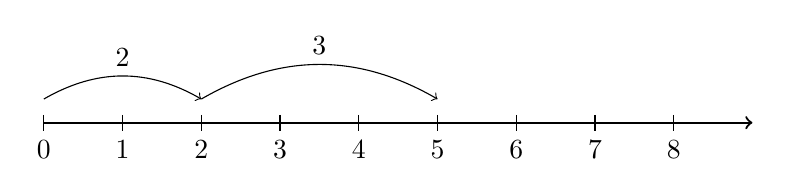
\begin{tikzpicture}
\draw[thick, ->] (0,0) -- (9,0) node[below] {$\ $};
\foreach \n in {0,1,2,3,4,5,6,7,8} {\draw (\n,0.1) -- (\n,-0.1) node[below] {$\n$};}
\draw[->, bend left=30] (0,0.3) to node[above] {$2$} (2,0.3);
\draw[->, bend left=30] (2,0.3) to node[above] {$3$} (5,0.3);
\end{tikzpicture}
\end{center}

And here is $5-3=2$:

\begin{center}
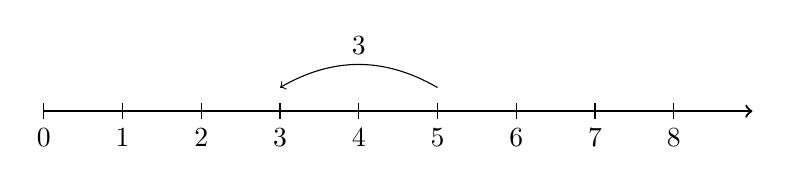
\begin{tikzpicture}
\draw[thick, ->] (0,0) -- (9,0) node[below] {$\ $};
\foreach \n in {0,1,2,3,4,5,6,7,8} {\draw (\n,0.1) -- (\n,-0.1) node[below] {$\n$};}
\draw[<-, bend left=30] (3,0.3) to node[above] {$3$} (5,0.3);
\end{tikzpicture}
\end{center}

The minuend has to be larger than the subtrahend or the difference will be less than zero, which is another subject.

\paragraph{The Subtraction Table}
Subtraction is the opposite of Addition. If you know your addition table for single-digit numbers then you also know how to subtract them.

\begin{center}
$5 + 3 = 8$, so $8 - 3 = 5$
\end{center}

\begin{table}[h]
\centering
\begin{tabular}{|l|l|l|l|l|l|l|l|l|l|}
\hline
- & 1 & 2 & 3 & 4 & 5 & 6 & 7 & 8 & 9 \\ \hline
1 & 0 & . & . & . & . & . & . & . & . \\ \hline
2 & 1 & 0 & . & . & . & . & . & . & . \\ \hline
3 & 2 & 1 & 0 & . & . & . & . & . & . \\ \hline
4 & 3 & 2 & 1 & 0 & . & . & . & . & . \\ \hline
5 & 4 & 3 & 2 & 1 & 0 & . & . & . & . \\ \hline
6 & 5 & 4 & 3 & 2 & 1 & 0 & . & . & . \\ \hline
7 & 6 & 5 & 4 & 3 & 2 & 1 & 0 & . & . \\ \hline
8 & 7 & 6 & 5 & 4 & 3 & 2 & 1 & 0 & . \\ \hline
9 & 8 & 7 & 6 & 5 & 4 & 3 & 2 & 1 & 0 \\ \hline
\end{tabular}
\caption*{The Subtraction Table}
\end{table}

\item Pick any two single-digit numbers and write an equation subtracting the smaller number from the larger number and showing their difference.
\item Which number is the minuend?
\item Which number is the subtrahend?
\item Which number is the difference?

\begin{table}[ht]
\centering
\begin{tabular}{|l|l|l|l|l|l|l|l|l|l|}
\hline
- & 1 & 2 & 3 & 4 & 5 & 6 & 7 & 8 & 9 \\ \hline
1 &  & . & . & . & . & . & . & . & . \\ \hline
2 &  &  & . & . & . & . & . & . & . \\ \hline
3 &  &  &  & . & . & . & . & . & . \\ \hline
4 &  &  &  &  & . & . & . & . & . \\ \hline
5 &  &  &  &  &  & . & . & . & . \\ \hline
6 &  &  &  &  &  &  & . & . & . \\ \hline
7 &  &  &  &  &  &  &  & . & . \\ \hline
8 &  &  &  &  &  &  &  &  & . \\ \hline
9 &  &  &  &  &  &  &  &  &  \\ \hline
\end{tabular}
\caption*{Blank Subtraction Table}
\end{table}

\item Fill in this blank subtraction table.

\subsection*{Subtraction in Columns}

Subtracting multi-digit numbers is done by arranging the numbers into columns aligned with the place-values all under each other. The ones, tens, hundreds and so on of each number should be under each other in vertical lines. Each column of digits is subtracted separately to get a difference that is written underneath.

\begin{center}
\begin{tabular}{c@{\,}c@{\,}c@{\,}}
 & &\text{ minuend}\\
$-$& &\text{ subtrahend}\\
\hline
=& &\text{ difference}\\
\hline
\hline
\end{tabular}
\end{center}

$72 - 21$ is $7 - 2 = 5$ and $2 - 1 = 1$, so that the difference of 51:

\begin{center}
\begin{tabular}{c@{\,}c@{\,}c@{\,}}
 &7&2\\
$-$&2&1\\
\hline
=&5&1\\
\hline
\hline
\end{tabular}
\end{center}

The difference is separated from the minuend and subtrahend by a single line, and is double underlined to show that this is a final answer.\\

Numbers, of any length, can be subtracted in this way, with the units, tens, thousands, and so on all aligned into columns to make the operation clear and simple.

\begin{center}
\begin{tabular}{c@{\,}c@{\,}c@{\,}c@{\,}c@{\,}c@{\,}c@{\,}c@{\,}}
  & &1&0&4,&2&1&3\\
 -& & & &3,&1&1&2\\
\hline
= & &1&0&1,&1&0&1\\
\hline
\hline
\end{tabular}\\
\end{center}

\item Subtract, in columns, 34 from 72.
\item Subtract, in columns, 4523 from 6721.

\subsubsection*{Borrowing}
In addition in columns we had the situation where a subtotal could be greater than 9 so that the 10s value had to be carried over to the next higher column.\\

We have the opposite problem in subtracting in columns. Sometimes the subtrahend is greater than the minuend so the difference would be less than 0. That's solved by borrowing from the next highest column.\\

Here, in the 1s column, you can't take 5 from 3 so you borrow from the 10s column. Cross out the 5 and make it a 4, and add that 10 to the 3 that now becomes 13. Now you can do $13-5=8$ and $4-1=3$ to get your difference.

\begin{center}
\begin{tabular}{c@{\,}c@{\,}c@{\,}c@{\,}c}
& & &^{4}\cancel{5}&^{1}3\\
   - & & &1&5\\
	\hline
	& & &3&8\\
	\hline
	\hline
\end{tabular}
\end{center}

Here is another longer example of subtraction:

\begin{center}
\begin{tabular}{c@{\,}c@{\,}c@{\,}c@{\,}c}
&^2\cancel{3},&^{13}\cancel{4}&^{14}\cancel{5}&^{1}6\\
   - & &7&8&9\\
	\hline
	&2,&6&6&7\\
	\hline
	\hline
\end{tabular}
\end{center}

As you can see, sometimes borrowing can get into chains of borrowing before the subtraction can be done.

\begin{center}
\begin{tabular}{c@{\,}c@{\,}c@{\,}c@{\,}c}
&^0\cancel{1},&^{9}\cancel{{^{1}0}}&^{9}\cancel{{{^1}0}}&^{1}0\\
   - & &7&8&9\\
	\hline
	&2,&6&6&7\\
	\hline
	\hline
\end{tabular}
\end{center}

Practice doing subtraction with borrowing:
\item What is 742 - 389?
\item What is 956 - 417?
\item What is 820 - 398?
\item What is 574 - 289?
\item What is 643 - 326?
\item What is 968 - 537?
\item What is 726 - 398?
\item What is 835 - 476?
\item What is 921 - 582?\\

\item Keep practicing subtracting numbers until you are getting right answers every time and you feel confident about it.\\

And that's how you do subtraction!

\vspace{16pt}
\subsection*{Adding and Subtracting\\by Equal Adjustment}
Sometimes when adding or subtracting two numbers it is easier to add or subtract a small amount to both numbers, to make the units digit equal to zero. You don't have to carry or borrow digits this way, which is easier, and with practice you can do it in you head without writing.\\

\paragraph{Adding}
For example, $78 + 96$ is the same as $78 + 2 + 96 - 2$. You are just adding two and taking it away again, leaving the sum unchanged. It is easier to add $80 + 94$ than to add $78 + 96$, but they both result in the same sum.\\

Add these numbers by adjusting:
\item 348 + 52
\item 176 + 124
\item 637 + 363
\item 829 + 171
\item 492 + 508

\paragraph{Subtracting}
In the same way, $96 - 78$ is the same as $96 + 2 - 78 + 2$. The difference remains the same. $98 - 80$ is a much easier problem to solve.

Subtract these numbers by adjusting:
\item 723 - 323
\item 957 - 457
\item 826 - 326
\item 513 - 113
\item 964 - 164

\subsection*{Checking Subtraction}

\paragraph{Adding upwards}
Subtraction can be checked by rearranging the numbers to make an addition. If $a-b=c$ then $c+b=a$. There is no need to write out the addition because the digits can be added upward mentally.\\

\item Subtract 3456 from 7296, and then check the difference by adding upwards. Did you get it right?

\paragraph{Casting out 9s and working out the digit sums}
Casting out 9s and finding digit sums can be done but is not as useful as for addition, where there may be a long list of numbers, because with subtraction you are usually only dealing with two numbers.\\

\begin{center}
\begin{tabular}{c@{\,}c@{\,}c@{\,}c@{\,}c}
& &1&^{4}\cancel{5}&^{1}3\\
   - & & &1&5\\
	\hline
	& &1&3&8\\
	\hline
	\hline
\end{tabular}
\end{center}

If the digit sum of the subtrahend is larger than the digit sum of the minuend, you can either add 9 to the minuend, or you can rearrange the subtraction into an addition.\\

The digit sum for 153 is $1+5+3 = 9 = 0$. Add 9 to make it larger than the subtrahend. The digit sum for 15 is $1 + 5 = 6$. The difference of these digit sums is $9 - 3 = 6$. The digit sum for 138, casting out 9s, is also 3, so the answer is probably correct.\\

\item Go back to the subtraction of 3456 from 7296 and this time check the difference by casting out 9s and working out the digit sums. Did you get it right?

\end{enumerate}

\end{document}
